\documentclass{article}

\usepackage[utf8]{inputenc}
\usepackage{graphicx}
\usepackage{float}
\usepackage{amsmath}

\linespread{1.6}
\addtolength{\textwidth}{20mm}
\addtolength{\oddsidemargin}{-10mm}
\linespread{1.6}
\addtolength{\textwidth}{20mm}
\addtolength{\oddsidemargin}{-10mm}

\begin{document}

\newtheorem{theorem}{Theorem}[section]
\newtheorem{definition}[theorem]{Definition}
\newtheorem{lemma}[theorem]{Lemma}
\newtheorem{observation}[theorem]{Observation}
\newtheorem{example}[theorem]{Example}
\newtheorem{corollary}[theorem]{Corollary}
\newtheorem{remark}[theorem]{Remark}
\newcommand{\eod}{$\quad\triangleleft$}
\newenvironment{defn}{\begin{definition}}{\hfill$\blacksquare$\end{definition}}
\newenvironment{defn*}{\begin{definition}}{\end{definition}}
\newenvironment{proof}{\noindent{\bf Proof.}}{\hfill$\blacksquare$}

\begin{titlepage}
\begin{picture}(250,530)(0,0)
\put(210,480){\makebox(0,0)[c]{\LARGE \bf ATILIM UNIVERSITY}}
\put(210,440){\makebox(0,0)[c]{\Large \bf DEPARTMENT of MATHEMATICS}}
\put(210,310){\makebox(0,0)[c]{\Large \bf MATH 411 Seminar Studies}}
\put(210,280){\makebox(0,0)[c]{\Large \bf Term Project Report}}
\put(210,240){\makebox(0,0)[c]{\Large \bf Title: Steganography and Its Applications:}}
\put(210,220){\makebox(0,0)[c]{\Large \bf An Application Using Least Significant Bit Method}}
\put(210,125){\makebox(0,0)[c]{\Large \bf Submitted by: Burcu ALAKUŞ}}
\put(210,100){\makebox(0,0)[c]{\Large \bf Instructor: Fatih SULAK}}
\put(210,000){\makebox(0,0)[c]{\Large \bf June, 2020}}
\end{picture}
\end{titlepage}


%DO NOT EDIT ABOVE THIS LINE EXCEPT FOR THE NAMES AND THE DATE


\tableofcontents
\newpage

\begin{flushright}
\begin{quote}
You can search and search, but when you've found nothing, you can only conclude: Maybe I didn't look hard enough, maybe there is nothing to find. (Clair, 2001)[1]
\end{quote}
\end{flushright}

	
	\section{Introduction}
	
There are two widely known ways to provide information security concepts such as "security, privacy, confidentiality, data integrity, accessibility" on issues such as secure communication, and information transmission. The first is cryptography and the other is steganography, that is, the method of data hiding. In both, the aim is to ensure that information is not learned by third parties, except only the sending and receiving parties. Accordingly, different methods, tools and concepts have been used and developed in both domains. While cryptography treats communication between the two parties as private and confidential, steganography provides the secrecy of communication.\\
\\
The way and method of cryptography is the process of transforming information with the values produced as a result of mathematical calculations in a way that the reader and the analyser cannot understand. Third parties cannot make sense of the message they have received message first, because the message has been changed. The message needs to be analysed and the analysis process requires a significant time and effort. The main idea of cryptography is to make it as hard as possible for third parties to resolve the message sent, to prevent them from understanding the original message if possible.\\
\\
In the other domain, Steganography, the purpose is not to take the precaution by transforming the message, but to send it by concealing the message completely. There are many methods and tools used to do that. The message is sent to a carrier hiding in a way that does not attract attention. In cryptography, although the message is encrypted, it is visible and attracts the attention and their interest of the parties; can be analyzed and encourages the decryption of encryption. When third parties reach the carrier, they will not be able to notice whether there is a message in their hands since they cannot notice a trace of the message and they are prevented from learning the message.\\
\\
It is thought that steganography techniques have been used in many fields throughout history, it is also known according to written sources. Steganography techniques can be used and was used in pre-war preparations, wars, political and diplomatic talks, intelligence activities (espionage), escapes from prison, riots and preparations. In the literature views section, today's modern applications of steganography will be discussed.
\subsection{Old Methods}The first written source mentions two events using steganography; in the Histories, the work of Heredotus (Herodotus, 484 BC - 425 BC) by the writer of Ancient Greece and historian Heredot. A message was written on the head by scraping the hair of a slave, when the hair grows again, the slave is sent to the place to be transmitted[2]. In this way, the message is reached the recipient without any attention. Another method is to write on wax tablets made of wood. When it was covered with wax once more, the text was hidden and sent[1].\\
\\
In 18th century, the war parties used invisible inks to communicate. Many liquids can be used as invisible ink. Secret messages written by using lemon juice, onion juice, milk, urine, juices and vinegar become darker when heated and hidden messages appear. Invisible inks used today emerge under ultraviolet light and are used against forgery[1].\\
\\
Many new techniques were used during the Second World War. With the development of photography, the Germans used the microdots technique. The message written in this technique is minimized to 200 times and above with photographic techniques, and brought to a point size and placed on a magazine, newspaper or any carrier[1]. It does not need to be encrypted. The reason to success with this methos is that it does not attract anyone's attention, because the messages sent are too small to be noticeable to the eye. This method is described by FBI manager J. Edgar Hoover as "The enemy's masterpiece of espionage."[3]\\
\\
Another technique used in this period is Null Cipher. The purpose of this method is to hide the message of any subject such as weather, shopping list, daily notes to a message that has no meaning. The message to be hidden is hidden to the carrier message in a sequential order, letter by letter. Many spies conveyed a lot of information with this method[4].
\\ 
\\
Also, in 2001 in Ron Howard's A Beautiful Mind, John Nash searches for hidden messages in newspapers and magazines[5].
\subsection{Application Areas}
With the development of the digital world, steganography also entered the digital world. With the Internet, an intense flow of information has taken place. The idea of moving data from one place to another has become very popular in the computer world, as in normal life. Over the World; texts, picture, sounds, video files are sent and received both compressed and uncompressed with the Internet.
\\
Today, there are multiple data hiding methods. Steganography is done by deleting redundant and noisy data fields in file formats and replacing hidden messages. The use of this method in the computer world is based on 2 main principles. The first is to embed data in the data, and the second is to hide the data in image or audio files. One of the main principles; The content of the image or audio files can be changed to some degree without harming the image or sound. The other principle is that the senses of a person cannot notice minor changes in image, sound or color.
\\
When analyzing a steganographic algorithm, 3 main features should be considered:\\
\indent• Change should not be noticeable\\
\indent• Amount of data that can be stored\\
\indent• Durability


\subsection{Techniques} 
The techniques used in steganography can be summarized as a list below:\\
	\indent• Text Steganography (Message Hiding in a Text)\\
	\indent• Acrostic (Initialization)\\
	\indent• Open Spaces Techniques\\
	\indent• Image Steganograpgy (Message Hiding in an Image\\
	\indent• Least Significant Bit Technique\\
	\indent• JPEG Algorithm (Discrete Cosine Transform (DCT))\\
	\indent• Bit-Plane Complexity Segmentation Based Steganography (BPCS)\\
	\indent• Masking and Filtering\\
	\indent• Audio Steganography (Message Hiding in an Audio)\\
	\indent• Message Hiding in TCP/IP Packages \\
	\indent• Message Hiding in HTML Pages\\
		
\subsection{Purpose} To implement an environment to use both cryptography algorithms and steganography together, where users can encrypt their messages and hide these messages in an image file. 
	
\subsection{Significance} 
Steganography is not an alternative to encryption, but a complement to it. It has emerged as a new encryption method in recent years. This approach can be briefly described as hiding data inside an object. Today's steganography techniques use audio, digital image or video files to hide encrypted data to further enhance security. While encrypted data draw attention on their own, they will not be attempted to be broken because nobody will notice when they are hidden inside the image or audio files.
	
\subsection{Implications} 
Steganography is a dynamic tool thanks to its deep-rooted history and structure that can keep pace with new technologies. Success in steganographic secrecy is achieved by choosing a suitable mechanism. The development in steganography continues day by day, and its usage areas are open to expansion over time. Its use will inspire many methods.
	
	\section{Literature Review}
	\indent In the literature, to increase the security of data while transmitting through network M. Indra Sena Reddy and Dr. A.P. Siva Kumar have used steganography and cryptography methods together [6]. They have used AES algorithm to encrypt the text to be sent, then embed this encrypted text in an image with the Least Significant Bit (LSB) method [6]. They have also extract encrypted text from transmitted resultant image and decrypt the text to get the original message[6].\\
\indent M. Jain, S.K. Lenka and S.K. Vasistha have used RSA cryptosystem in adaptive circular queue image steganoraphy [7]. The data structure queue is employed to resource distribution and RSA cryptosystem is used for secret information confidentiality and authentication [2]. They get higher results as compared with several of existing algorithms of image steganography.\\
\indent In another paper, P.Sethi, V. Kapoor have proposed and architecture for information hiding in image steganography by using genetic algorithm and cryptography [8]. They have used AES cryptographic algorithm to get cipher text and genetic algorithm for pixel assortment of image where the data is to be concealed [8].\\
R. Bhardwaj and V. Sharma have used steganography based on complemented messages and inverted LSB substitution where pixels are selected randomly when embedding the message [9]. This reduces the chance of detection of hidden message.\\

As it is seen in the literature, this study has a novel part. Finding a way of combining different techniques from previous studies, is needed to be done.

\section{RSA \& AES}

Encryption is a process of taking a message and scrambling its contents so that only certain people can look at that message. There are two types of encryption: symmetric and asymmetric encryption.\\
To understand why asymmetric encryption was created, first we need to look at symmetric encryption. To do that, we should think about two people: Alice and Bob. Alice has a sensitive document that she wants to share with Bob. She uses an encryption program to protect her document with a passphrase that she chooses. She then sends the encrypted document to Bob. However, Bob cannot open this message because he doesn't know the passphrase that Alice used to encrypt the document. In other words: he doesn't have the key to open the lock.\\
How does Alice share this passphrase securely with Bob? Sending it through e-mail is risky because others might find the passphrase and use it to decrypt any messages between Alice and Bob. In public key encryption, we need two keys; one is public key and another is secret key. These two are mathematically depends on each other. RSA consists of three steps (see Figure 1.):\\\\
\indent \textbf{1. Generating key}\\
\indent\indent • Two large enough prime numbers are selected, say \textbf{p} and \textbf{q}.\\
\indent\indent • \textbf{n} is computed as\textbf{ n=p.q}\\
\indent\indent • Toitent function is computed as \textbf{$\phi$(n)=(p-1).(q-1)}\\
\indent\indent • A prime \textbf{e} number is selected such that \textbf{gcd($\phi$,e)=1} and \textbf{1 $<$ e $<$ $\phi$}. \indent\indent   This \textbf{e} number is said to be the public key.\\
\indent\indent • Then, a \textbf{d} number is computed as \textbf{d.e$\equiv$1 (mod $\phi$(n))}.  \\
\indent\indent   Here the \textbf{d} number is said to be the private key.\\\\
We have generated the keys. Now, we will encrypt the message.\\\\
\indent \textbf{2. Message Encryption}\\
\indent\indent • For encryption Bob sends his public key as \textbf{(n,e)}.\\
\indent\indent • Alice encrypts her message as \textbf{c$\equiv$m$^{e}$(mod n)}\\\\
\indent \textbf{3. Message Decryption}\\
\indent\indent • For decrypt the message, Bob calculates \textbf{m$\equiv$c$^{d}$(mod n)}, and gets message \textbf{m}. \\
\begin{center}
\begin{figure}[h]
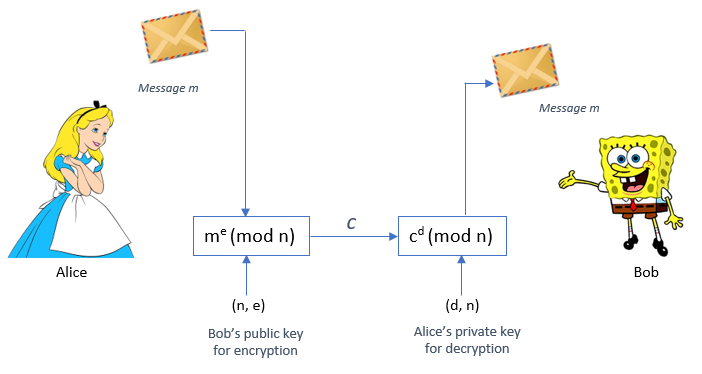
\includegraphics[width=9cm, height=4.5cm]{rsa}
\centering
\caption{RSA Encryption \& Decryption}
\end{figure}
\end{center}
AES stands for Advanced Encryption Standard and is in wide use around the world. It is a “symmetric” encryption method, where the same secret (an encryption key) is used to encrypt the data, and also used to decrypt the data. It is an iterative method. It comprises of a series of linked operations, some of which involve replacing inputs by specific outputs (substitutions) and others involve shuffling bits around (permutations).\\
AES does its computations on bytes. 128 bits of a plaintext block is treated as 16 bytes with AES standard. These 16 bytes are arranged in four columns and four rows for processing as a matrix. AES uses 10 rounds for 128-bit keys, 12 rounds for 192-bit keys and 14 rounds for 256-bit keys. Each of these rounds uses a different 128-bit round key, which is calculated from the original AES key[10].
\begin{center}
\begin{figure}[!htbp]
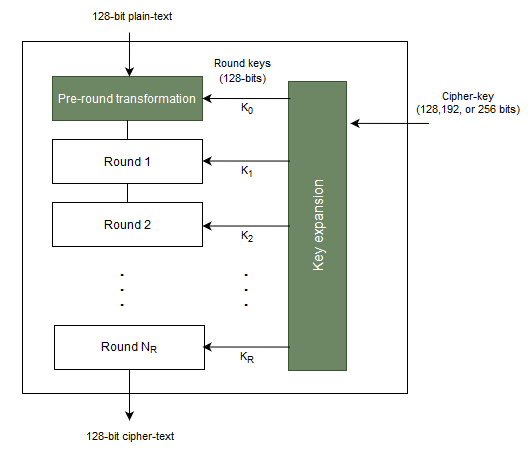
\includegraphics[width=10cm, height=7cm]{aes1}
\centering
\caption{AES Encryption Structure}
\end{figure}
\end{center}
\subparagraph{Encryption Process}\mbox{}\\
Here is the typical description of round in AES encryption. Each round comprise of four sub-processes. The first round process is shown below:
\begin{center}
\begin{figure}[h]
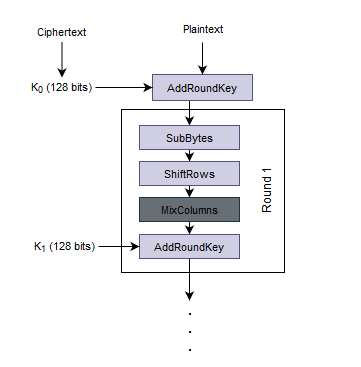
\includegraphics[width=6cm, height=5.5cm]{aes2}
\centering
\caption{AES Encryption Process of a Round}
\end{figure}
\end{center}
• \textbf{Byte Substitution (SubBytes)}\\

The 16 input bytes are substituted by looking up a fixed table (S-box) given in design. The result is a 4x4 matrix.\\
\newpage
• \textbf{Shiftrows}\\

Each of the four rows of the matrix is shifted to the left. Any entries that ‘fall off’ are re-inserted on the right side of row. Shift is carried out as follows:\\

    \indent\indent   First row is not shifted.\\
    \indent\indent   Second row is shifted one (byte) position to the left.\\
    \indent\indent   Third row is shifted two positions to the left.\\
    \indent\indent   Fourth row is shifted three positions to the left.\\

    The result is a new matrix consisting of the same 16 bytes but shifted with respect to each other.\\

• \textbf{Mixcolumns}\\

Each four-byte column is now converted using a special mathematical function. This function takes four bytes of a column as input and returns a completely new four byte that replaces the original column. The result is another new matrix consisting of 16 new bytes. This step was not carried out in the last round.\\

• \textbf{AddRoundKey}\\

The 16 bytes of the matrix are now considered as 128 bits and are converted to 128 bits of the round key with XOR. If this is the last round, the output is cipher text. Otherwise, the resulting 128 bits are interpreted as 16 bytes and we start another round.\\\\
\newpage
\subparagraph{Decryption Process}

\begin{center}
\begin{figure}[h]
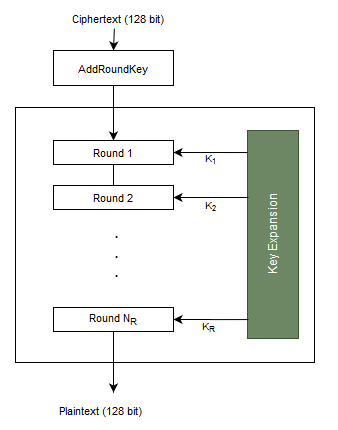
\includegraphics[width=7cm, height=7.5cm]{aes3}
\centering
\caption{AES Encryption Structure}
\end{figure}
\end{center}

The process of decryption of an AES is similar to the encryption process in the reverse order. Each round consists of the four processes in the reverse order:\\

    \indent \indent Add round key\\
    \indent \indent Mix columns\\
    \indent \indent Shift rows\\
    \indent \indent Byte substitution

\begin{center}
\begin{figure}[H]
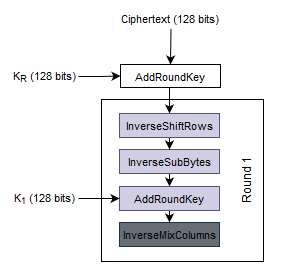
\includegraphics[width=4.5cm, height=4cm]{aes4}
\centering
\caption{AES Decryption Process of a Round}
\end{figure}
\end{center}

\section{Least Significant Bit (LSB) Method}
Formally a stegosystem consists of triplet that generates keys, encodes the message and decodes the message. Stegosytem (see Figure 6) contains the following components:\\
\\emb: message to be embedded\\
\\cover: file to embed the data\\
\\stego: modified version of the cover containing an embedded message\\
\\key: extra confidential data required for embedding and opening operations, which should also be known to the sender and receiver\\
\\f\textsubscript{E}: a steganographic function with key, emb and cover as parameter and generating stego as output\\
\\f\textsubscript{E}\textsuperscript{-1}: a steganographic function that has a stego with key as a parameter and generates emb as an output. f\textsubscript{E}\textsuperscript{-1} is the inverse function of f\textsubscript{E}.
\begin{figure}[h]
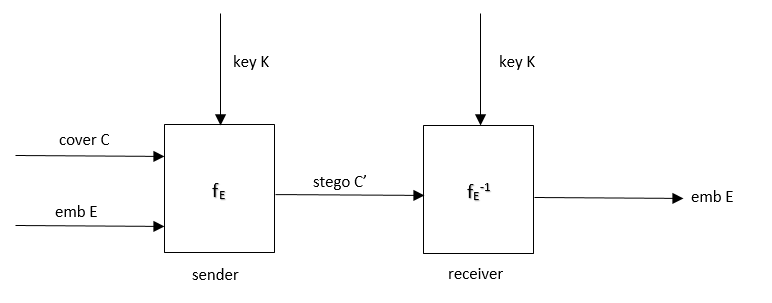
\includegraphics[width=12cm, height=4cm]{sego}
\centering
\caption{Formal Stegosystem}
\end{figure}
\\The sender creates a steganogram using a hiding function. The hiding function has two parameters, the carrier cover where the data will be stored and the data to be hidden [11].
\begin{figure}[H]
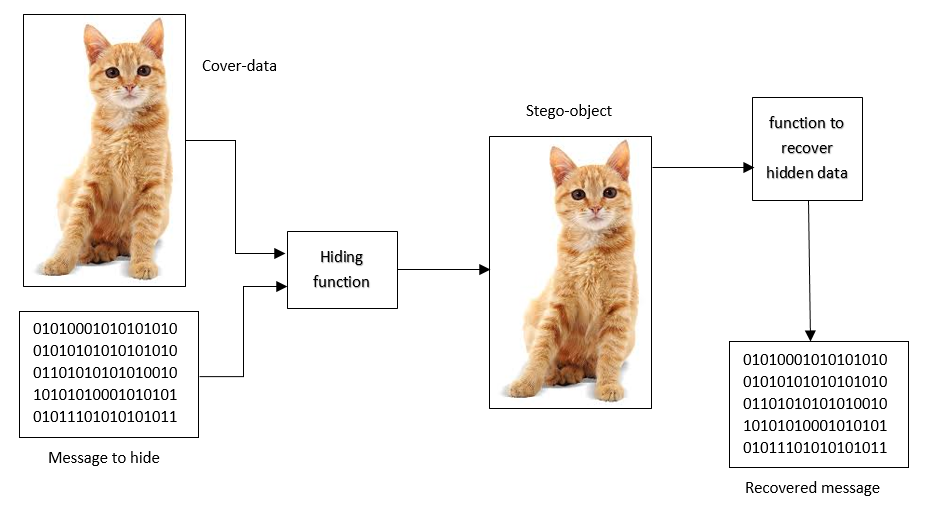
\includegraphics[width=13.5cm, height=6.5cm]{stego2}
\centering
\caption{Image Stegosystem}
\end{figure}
In image steganography, there are various methods for hiding information in an image. These methods, called Hiding Function (see Figure 7), are listed below [13]:\\
\indent \indent • LSB\\
\indent \indent • Masking and Filtering\\
\indent \indent • Algorithms \& Transformations

\subparagraph{LSB Algorithm Example [13]}\mbox{}\\
	
\textbf{• Algorithm to embed text message:}\\
\indent \indent Step 1: Read the cover image and text message which is to be hidden in the cover image.\\
\indent \indent Step 2: Convert text message in binary\\
\indent \indent Step 3: Calculate LSB of each pixels of cover image.\\
\indent \indent Step 4: Replace LSB of cover image with each bit of secret message one by one.\\
\indent \indent Step 5: Write stego image.\\
\indent \indent Step 6: Calculate the Mean Square Error (MSE), Peak signal to noise ratio (PSNR) of the stego image.\mbox{}\\\\
\textbf{• Algorithm to retrieve text message:}\\
\indent \indent Step 1: Read stego image.\\
\indent \indent Step 2: Calculate LSB of each pixels of stego image.\\
\indent \indent Step 3: Retrieve bits and convert each 8 bit into character.\\


\section{Methods Used In This Project}
\subsection{Coding of The Application}In this project Least Significant Bit method is used to embed text or image into a carrier image. To do that Python programming language is selected. Since we are dealing with images, OpenCV (Open Source Computer Vision Library) is used. Also, we have array computations, so, NumPy library is selected to operate these arrays. Finally, docopt library is used to create an interface for command-line app and parse the code automatically.\\
As it is mentioned before, in this project LSB method has been used. This technique is using picture's pixel information. This technique works best when the file is longer than the message file and if image is grayscale. When applyin LSB techniques to each byte of a 24 bit image, three bits can be encoded into each pixel.\\
\begin{figure}[h]
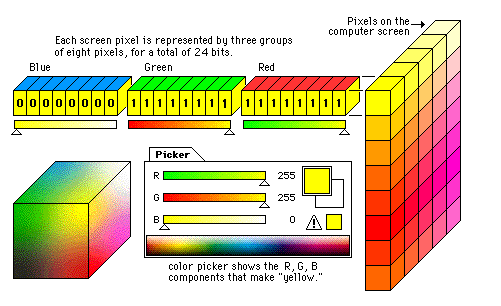
\includegraphics[width=12cm, height=6cm]{24bit}
\centering
\caption{Bitmap Colour Depth}
\end{figure}
\subsection{Algorithms for Message Embedding and Extracting}
If the LSB of the pixel value of cover image C(i,j) is equal to the message bit SM of secret message to be embedded, C(i,j) remain unchanged; if not, set the LSB of C(i,j) to SM.\\
Message embedding procedure is given below:
$$
S(i,j) = \left\{
        \begin{array}{ll}
            C(i,j)-1 & \quad $LSB(C(i,j))=1$ $ and$ $ SM=0$ \\
             C(i,j)+1 & \quad $LSB(C(i,j))=0$ $ and$ $ SM=1$ \\
              C(i,j) & \quad $LSB(C(i,j))=SM$
        \end{array}
    \right.
$$
where LSB(C(i,j)) stands for the LSB of the cover image C(i,j) and "SM" is the next message bit to be embedded. S(i,j) is the stego image.\\
The algorithm used in the code for embedding is given below:
\begin{itemize}
\item Step 1: Extract the pixels of the cover image.
\item Step 2: Extract the character of the text or the pixels of the image.
\item Step 3: Extract the length of the secret message. (Length coded on 2 bytes so the text size can be up to 65536 bytes long)
\item Step 4: Choose first pixel and embed length of the secret message in the first 2 bytes pixels.
\item Step 5: Skip to the pixels after the length bytes.
\item Step 6: Insert characters of the message text in each component of next pixels by replacing it.
\item Step 7: Repeat step 6 till all the characters has been embedded.\\\\
\end{itemize}
Message extracting procedure is given below:
$$
SM = \left\{
        \begin{array}{ll}
            0  & \quad $S(i,j)=0$\\
            1  & \quad $S(i,j)=1$ 
        \end{array}
    \right.
$$
where "SM" is the message bit has been embedded. S(i,j) is the stego image.\\
For data extracting, steps below are used in the code:
\begin{itemize}
\item Step 1: Extract the pixels of the stego image.
\item Step 2: Start from first pixel and extract length of the message from first 2 bytes components of the pixels. 
\item Step 3: Skip to the pixels after the length bytes.
\item Step 4: Extract secret message bits from the pixels.
\item Step 5: Repeat step 4 till reach the pixels of length of the message.
\item Step 6: Decode message.
\end{itemize}
Here, every 4 bit-block represents an ASCII character, so it is easy to decode from ASCII to message character.
\subsection{The Application}
The application has two sides. One for embedding text and one for extracting the text. To embed text, you need to upload a cover image and then upload a text file. The program will create the stego image. For extracting, you need to select stego image to extract secret text message. The program will extract the message from the stego image and create the original message file.[see Figure 9]
\begin{figure}[h]
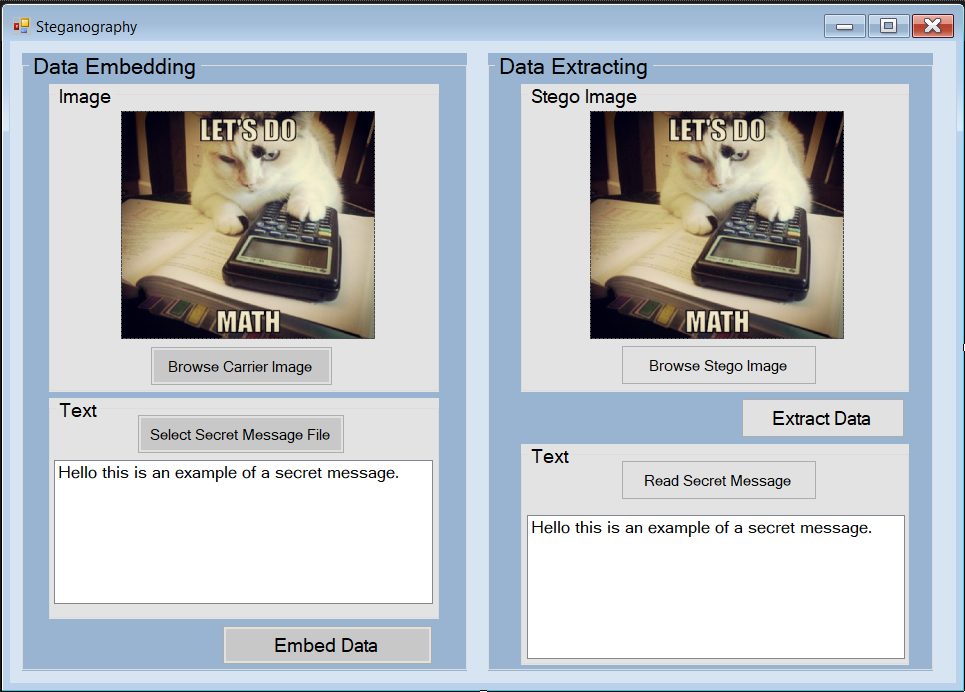
\includegraphics[width=14.5cm, height=10cm]{app}
\centering
\caption{Application screen}
\end{figure}

\newpage

\section{Conclusion \& Discussion}
The work proposed in this paper can be summarized with the following points:
\begin{enumerate}
\item Steganography and its history with old methods have been presented. 
\item The application areas for steganography has been mentioned.
\item Some techniques used for steganography have been listed.
\item Purpose, significance and implications of this project have been discussed.
\item Some literature review has done. 4 papers have been mentioned and these papers are about using steganography with cryptography. 
\item RSA and AES have been explained with their basic principles.
\item Least Significant Bit (LSB) method and information about one of an example algorithm was given.
\item Methods used in this project have been summarized and finally a conclusion and discussion part have been placed in this report.
\end{enumerate}
In this project, I wanted to use steganography with cryptography methods, but up to this time I have not been able to combine these two methods. So, this is left as a future work from now on. But LSB method for secret text/image embedding into an image worked properly.
\newpage
\section{References}
	\textbf{[1]} Clair, B. (2001). StrangeHorizons, 2020, Steganography, retrieved from http://strangehorizons.com/non-fiction/articles/steganography-how-to-send-a-secret-message/ \\\\
	\textbf{[2]} Herodotus; Sélincourt, Aubrey de, Translator (1954). The Histories. London: Penguin Books.Book V Chapters 33-35 \\\\
	\textbf{[3]} Microdot. 3 April 2020, retrieved from https://en.wikipedia.org/wiki/Microdot.  Hoover, J. Edgar (1946). "The enemy's masterpiece of espionage". Reader's Digest. 48 (April): 1-6. \\\\
	\textbf{[4]} Gaines, Helen F. (2014). Cryptanalysis: A Study of Ciphers and Their Solution. Courier Corporation. pp. 4–5. ISBN 9780486800592.\\\\
	\textbf{[5]} Das, R. (2013). Drain the Main Brain, 2020, Steganography – Hiding in Plain Sight, retrieved from \\https://drainthemainbrain.wordpress.com/2013/02/05/steganography-hiding-in-plain-sight/ \\\\
	\textbf{[6]} Reddy, I.S., Kumar. A.P.S. (2016), Secured Data Transmission Using Wavelet Based Steganography and Cryptography by Using AES Algorithm. International Conference on Computational Modeling and Security (CMS 2016). doi: 10.1016/j.procs.2016.05.177 \\\\
	\textbf{[7]} Jain, M., Lenka, S.K., Vasistha, S.K. (2016), Adaptive circulat queue image steganography with RSA cryptosystem. Recent Trends in Engineering and Material Sciences. doi: 10.1016/j.pics.2016.04.093\\\\
	\textbf{[8]} Sethi, P., Kapoor, V. (2016), A Proposed Novel Architecture for Information Hiding in Image Steganography by using Genetic Algorithm and Cryptography. 2016 International Conference on Computational Science.\\ doi: 10.1016/j.procs.2016.05.127\\\\
	\textbf{[9]} Bhardwaj, R., Sharma, V. (2016), Image Steganography Based on Complemented Message and Inverted bit LSB Substitution\\\\
	\textbf{[10]} Biclique Cryptanalysis of the Full AES (2016), retrieved from \\https://web.archive.org/web/20160306104007/http://research.microsoft.com/en-us/projects/cryptanalysis/aesbc.pdf\\\\
	\textbf{[11]} Westfield, Pfitzmann, A. (1999). Attacks on Steganographic Systems, Proceedings of Information Hiding - 3rd International Workshop, Springer Verlag, pp.61-67\\\\
	\textbf{[12]} Mishra, M., Mishra, P., Adhikary, M.C. (2012), Digital Image Data Hiding Techniques: A Comparative Study, ANVESA - The Journal of F.M. University, ISSN-0974-715X\\\\
	\textbf{[13]} Goel, S., Rana, A., Kaur, M. (2013), A Review of Comparison Techniques of Image Steganography, Global journal of computer science and technology, doi:10.9790/1676-0614148\\\\
		
	
	
\end{document}